\pagebreak
\section{Analiza zbiorów danych}

\subsection{Zbiór danych -- "Diabetes"}
\begin{table}[H]
  \center
  \begin{tabular}{|c|c|c|} \hline
    Nazwa klasy & Liczba instancji & \% instancji \\ \hline
    1 (chory) & 500 & 65 (\%)\\ \hline
    0 (zdrowy) & 268 &  35 (\%)\\ \hline 
  \end{tabular}
  \caption{Udział procentowy klas w zbiorze "Diabetes".}
\end{table}

\begin{table}[H]
\center
\begin{tabular}{|c|c|c|c|c|c|}
\hline
          Nazwa atrybutu  &   Min &   Max & Średnia & Ochyl. stand. & Rozkład \\ \hline
                  Glucose &     0 &   199 &  120.89 &   31.95 & 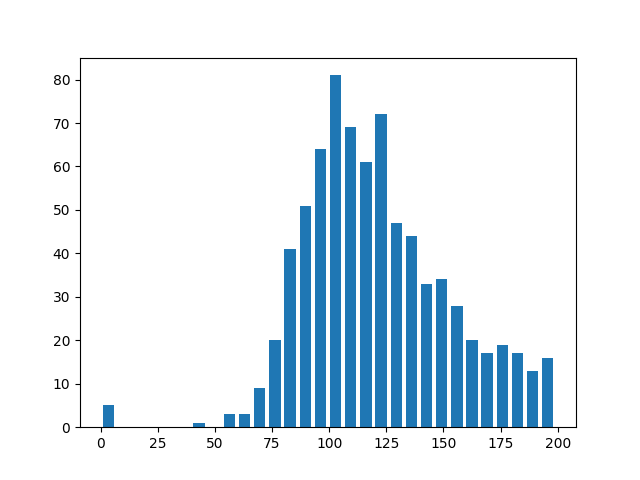
\includegraphics[width=0.2\textwidth]{img/stats/Glucose.png} \\ \hline
            BloodPressure &     0 &   122 &   69.11 &   19.34 & 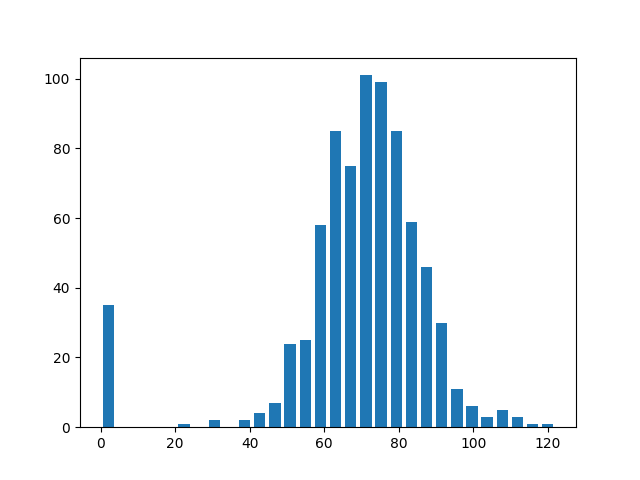
\includegraphics[width=0.2\textwidth]{img/stats/BloodPressure.png} \\ \hline
            SkinThickness &     0 &    99 &   20.54 &   15.94 & 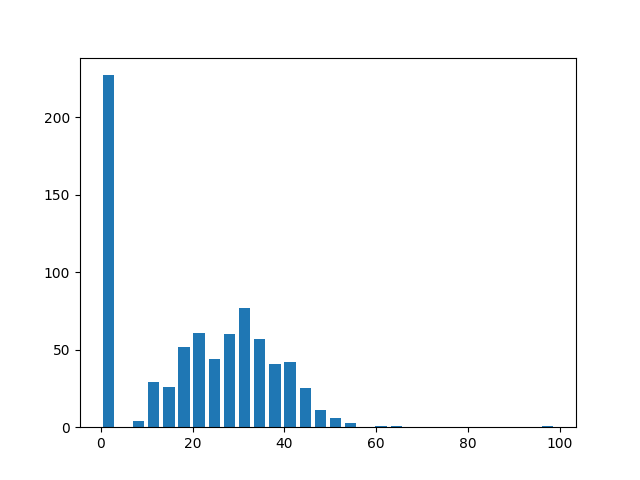
\includegraphics[width=0.2\textwidth]{img/stats/SkinThickness.png} \\ \hline
                  Insulin &     0 &   846 &   79.80 &  115.17 & 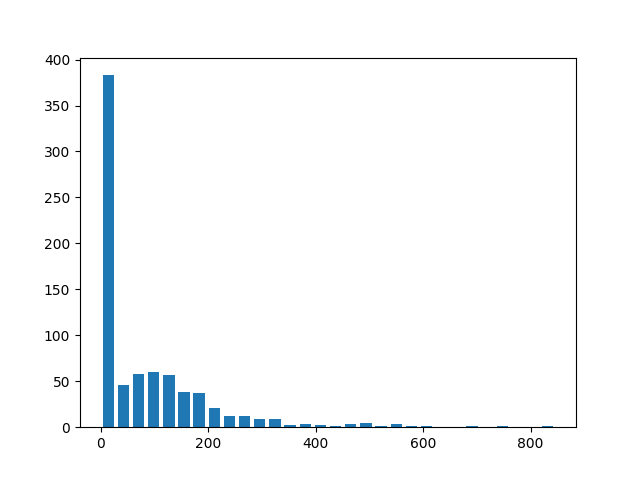
\includegraphics[width=0.2\textwidth]{img/stats/Insulin.png} \\ \hline
                      BMI &     0 &  67.1 &   31.99 &    7.88 & 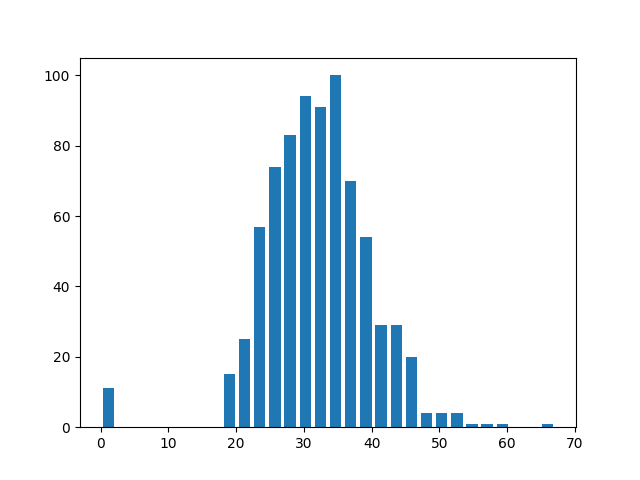
\includegraphics[width=0.2\textwidth]{img/stats/BMI.png} \\ \hline
 DiabetesPedigreeFunction &  0.08 &  2.42 &    0.47 &    0.33 &  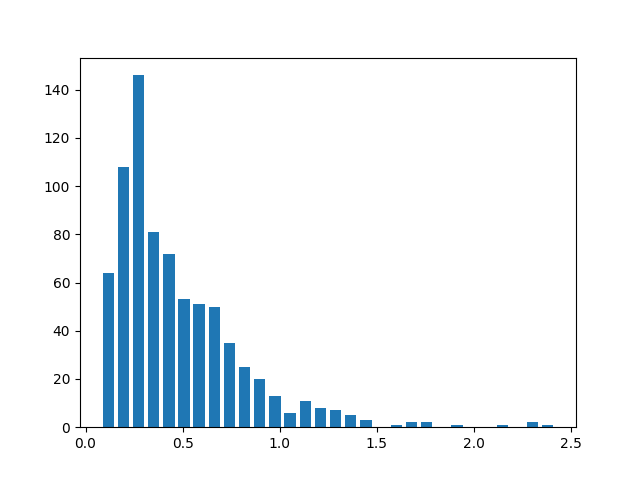
\includegraphics[width=0.2\textwidth]{img/stats/DiabetesPedigreeFunction.png} \\ \hline
                      Age &    21 &    81 &   33.24 &   11.75 & 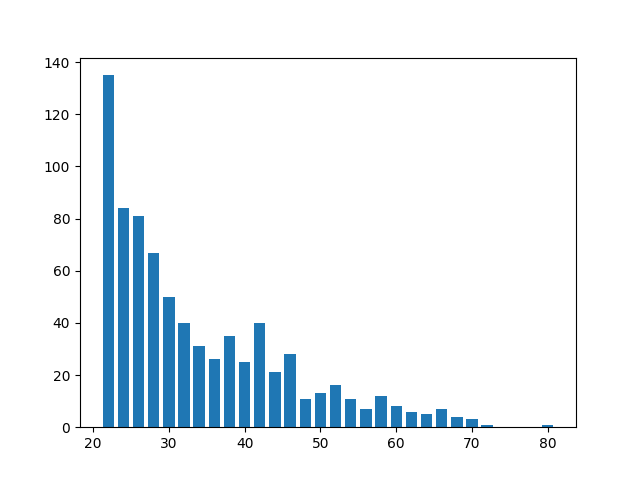
\includegraphics[width=0.2\textwidth]{img/stats/Age.png} \\ \hline
\end{tabular}
\caption{Atrybuty zbioru danych "Diabetes".}
\end{table}


\subsection{Zbiór danych -- "Glass"}
\begin{table}[H]
  \center
  \begin{tabular}{|c|c|c|} \hline
    Nazwa klasy & Liczba instancji & \% instancji \\ \hline
    1 (building\_windows\_float\_processed)       & 70 & 33 (\%)\\ \hline
    2 (building\_windows\_non\_float\_processed)  & 76 & 36 (\%)\\ \hline
    3 (vehicle\_windows\_float\_processed)        & 17 & 8 (\%)\\ \hline
    4 (vehicle\_windows\_non\_float\_processed)   & 0  & 0  (\%)\\ \hline
    5 (containers)                                & 13 & 6 (\%)\\ \hline
    6 (tableware)                                 & 9  & 4 (\%)\\ \hline
    7 (headlamps)                                 & 29 & 13 (\%)\\ \hline
    
  \end{tabular}
  \caption{Udział procentowy klas w zbiorze "Glass".}
\end{table}

\begin{table}[H]
  \center
  \begin{tabular}{|c|c|c|c|c|c|} \hline
Name &    Min &    Max &   Mean &   Std &        Distribution \\ \hline
  RI &   1.51 &   1.53 &   1.52 &  0.00 &  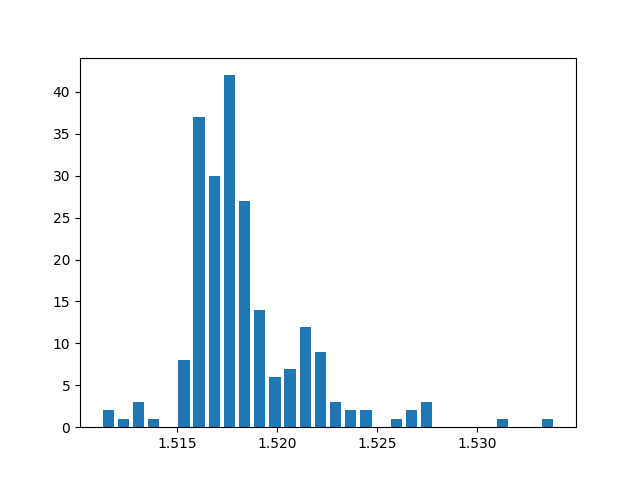
\includegraphics[width=0.2\textwidth]{img/stats/RI.png} \\ \hline
  Na &  10.73 &  17.38 &  13.41 &  0.81 &  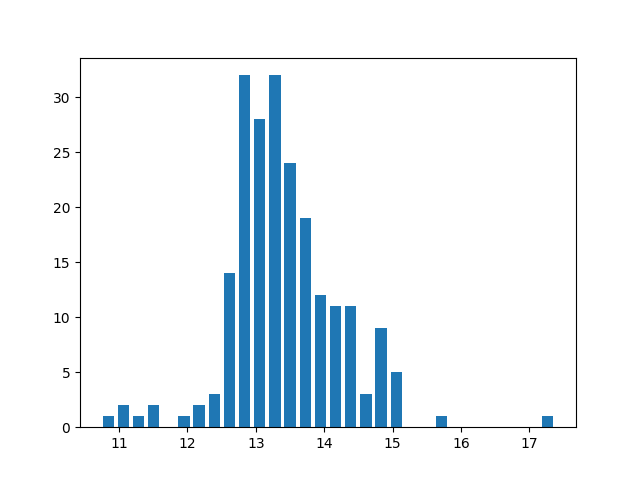
\includegraphics[width=0.2\textwidth]{img/stats/Na.png} \\ \hline
  Mg &   0.00 &   4.49 &   2.68 &  1.44 &  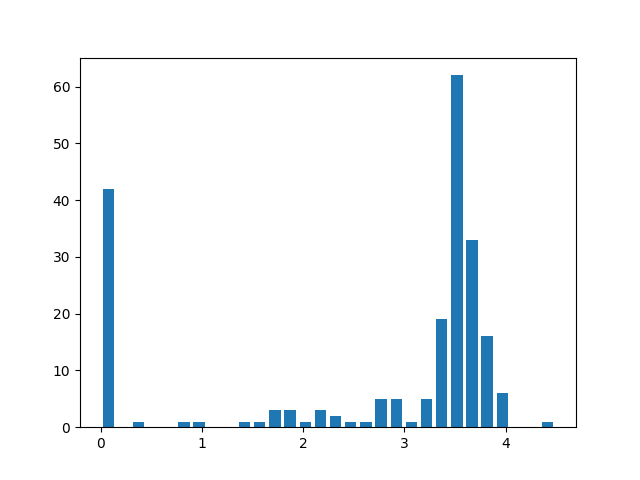
\includegraphics[width=0.2\textwidth]{img/stats/Mg.png} \\ \hline
  Al &   0.29 &   3.50 &   1.44 &  0.50 &  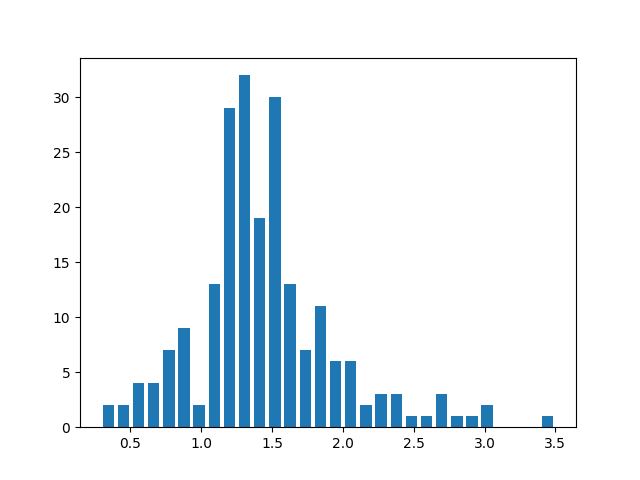
\includegraphics[width=0.2\textwidth]{img/stats/Al.png} \\ \hline
  Si &  69.81 &  75.41 &  72.65 &  0.77 &  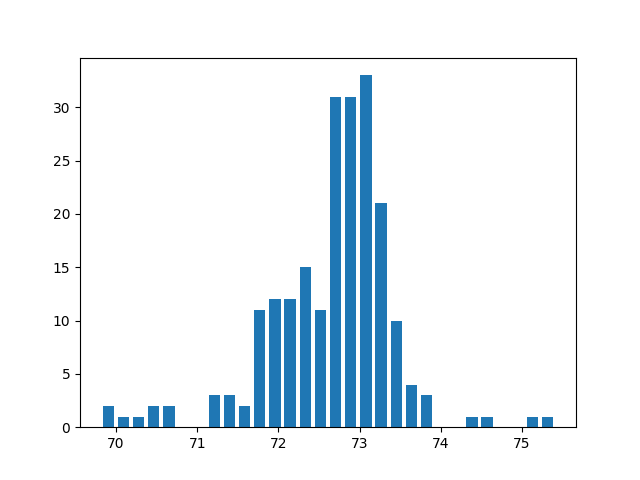
\includegraphics[width=0.2\textwidth]{img/stats/Si.png} \\ \hline
   K &   0.00 &   6.21 &   0.50 &  0.65 &   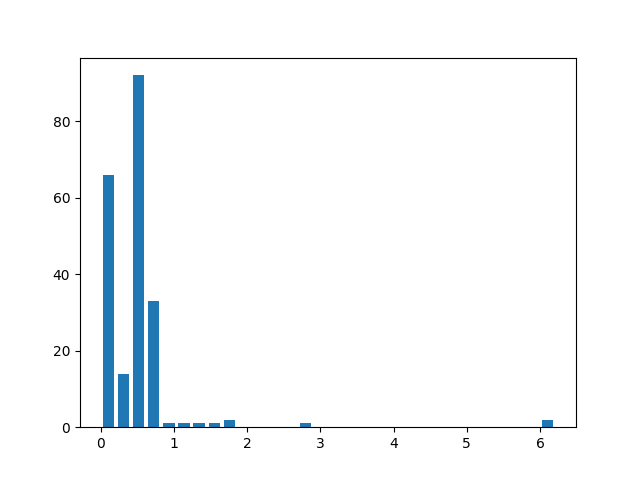
\includegraphics[width=0.2\textwidth]{img/stats/K.png} \\ \hline
\end{tabular}
\end{table}

\begin{table}[H]
  \center
  \begin{tabular}{|c|c|c|c|c|c|} \hline
  Ca &   5.43 &  16.19 &   8.96 &  1.42 &  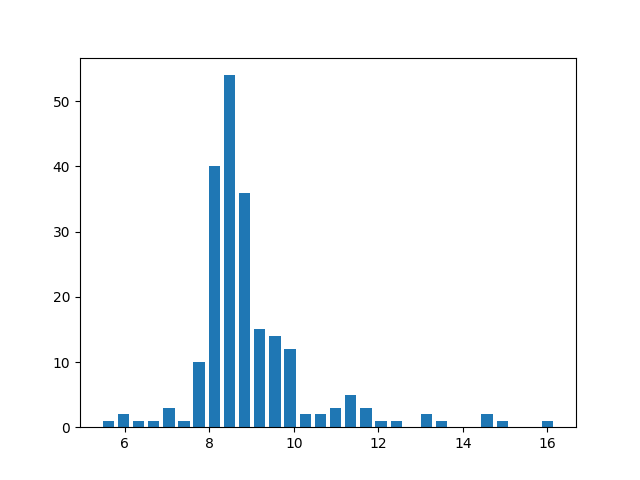
\includegraphics[width=0.2\textwidth]{img/stats/Ca.png} \\ \hline
  Ba &   0.00 &   3.15 &   0.18 &  0.50 &  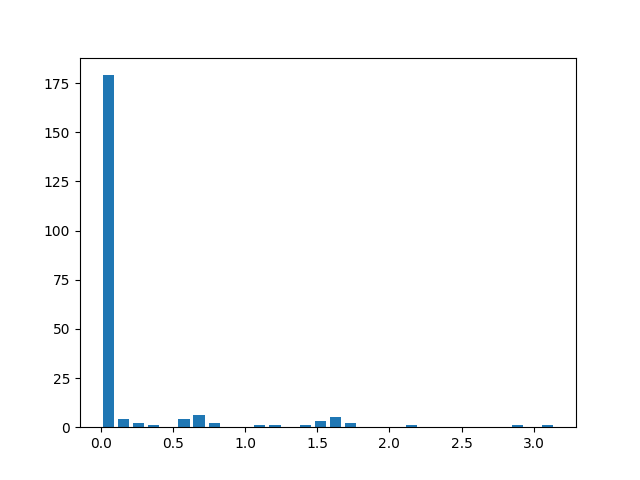
\includegraphics[width=0.2\textwidth]{img/stats/Ba.png} \\ \hline
  Fe &   0.00 &   0.51 &   0.06 &  0.10 &  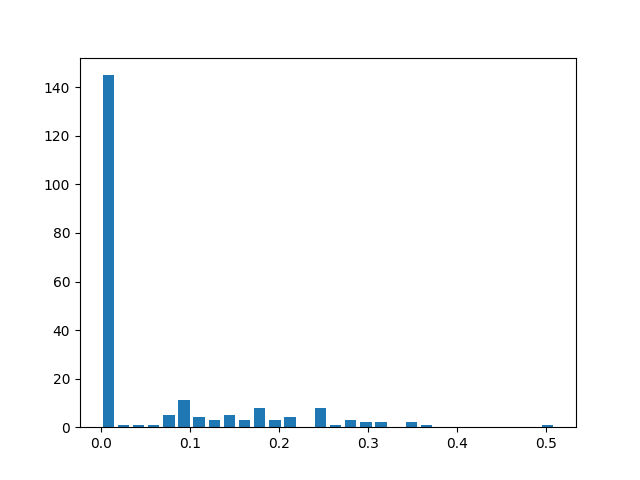
\includegraphics[width=0.2\textwidth]{img/stats/Fe.png} \\ \hline
\end{tabular}
  \caption{Atrybuty zbioru danych "Glass".}
\end{table}

\pagebreak
\subsection{Zbiór danych -- "Wine"}

\begin{table}[H]
  \center
  \begin{tabular}{|c|c|c|} \hline
    Nazwa klasy & Liczba instancji & \% instancji \\ \hline
    1 (Class 1)  & 59 & 33 (\%)\\ \hline
    2 (Class 2)  & 71 & 40 (\%)\\ \hline
    3 (Class 3)  & 48 & 27 (\%)\\ \hline
  \end{tabular}
  \caption{Udział procentowy klas w zbiorze "Wine".}
\end{table}


\begin{table}[H]
  \center
 \begin{tabular}{|c|c|c|c|c|c|} \hline
                 Name &     Min &      Max &    Mean &     Std &                          Distribution \\ \hline
              Alcohol &   11.03 &    14.83 &   13.00 &    0.81 &               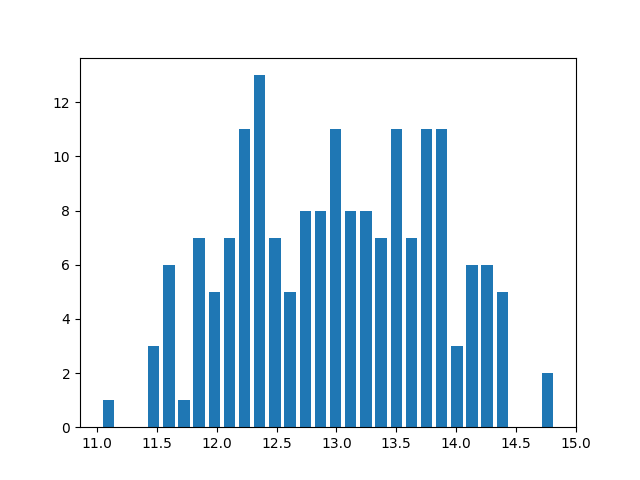
\includegraphics[width=0.2\textwidth]{img/stats/Alcohol.png} \\ \hline
           Macil\_acid &    0.74 &     5.80 &    2.34 &    1.11 &            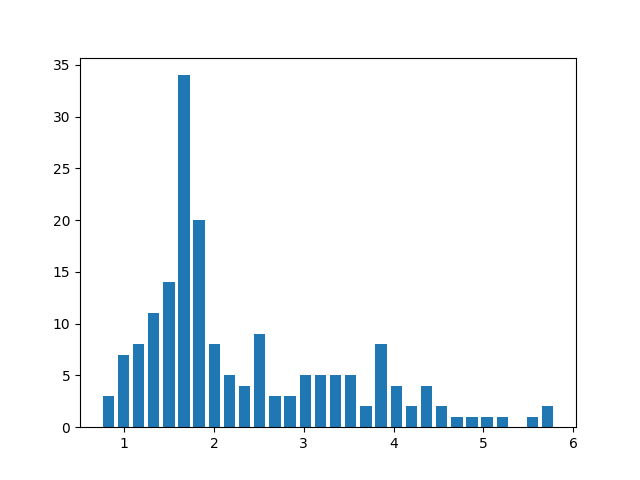
\includegraphics[width=0.2\textwidth]{img/stats/Macil_acid.png} \\ \hline
                  Ash &    1.36 &     3.23 &    2.37 &    0.27 &                   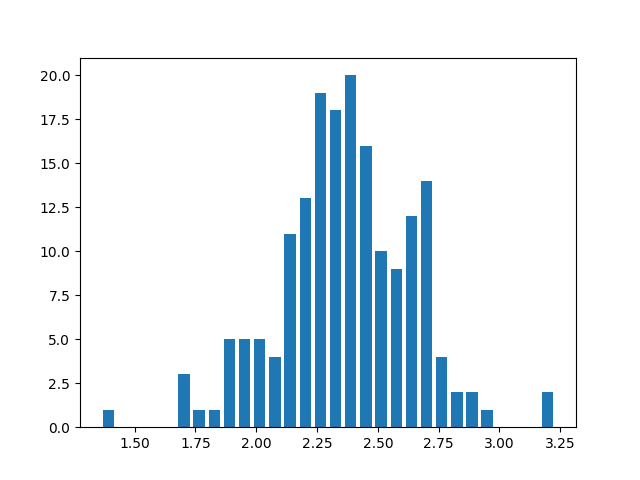
\includegraphics[width=0.2\textwidth]{img/stats/Ash.png} \\ \hline
    Alcalinity\_of\_ash &   10.60 &    30.00 &   19.49 &    3.33 &     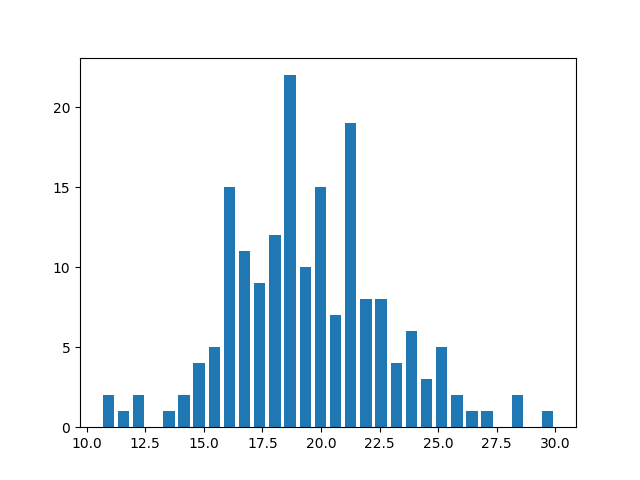
\includegraphics[width=0.2\textwidth]{img/stats/Alcalinity_of_ash.png} \\ \hline
            Magnesium &   70.00 &   162.00 &   99.74 &   14.24 &             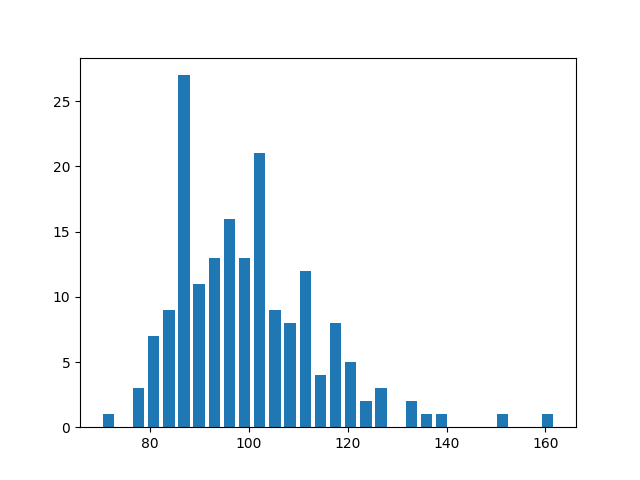
\includegraphics[width=0.2\textwidth]{img/stats/Magnesium.png} \\ \hline
        Total\_phenols &    0.98 &     3.88 &    2.30 &    0.62 &         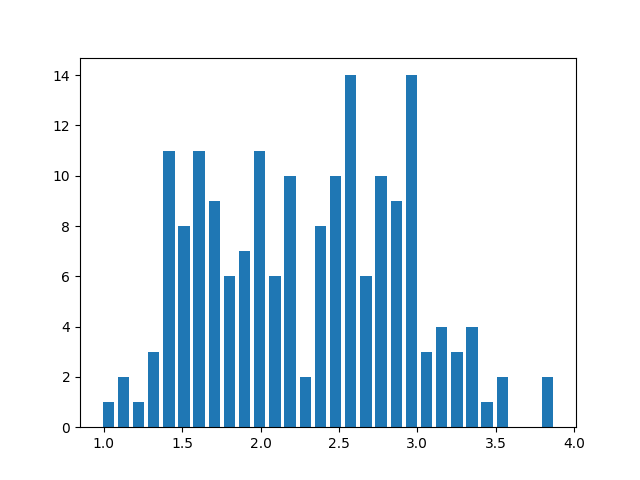
\includegraphics[width=0.2\textwidth]{img/stats/Total_phenols.png} \\ \hline
\end{tabular}
\end{table}

\begin{table}[H]
  \center
 \begin{tabular}{|c|c|c|c|c|c|} \hline
           Flavanoids &    0.34 &     5.08 &    2.03 &    1.00 &            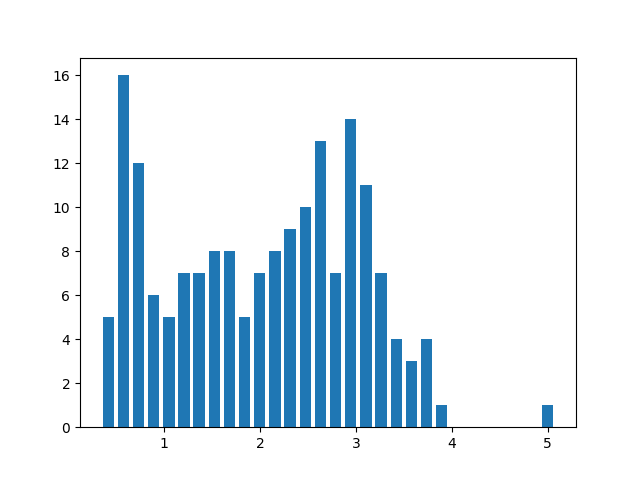
\includegraphics[width=0.2\textwidth]{img/stats/Flavanoids.png} \\ \hline
 Nonflavanoid\_phenols &    0.13 &     0.66 &    0.36 &    0.12 &  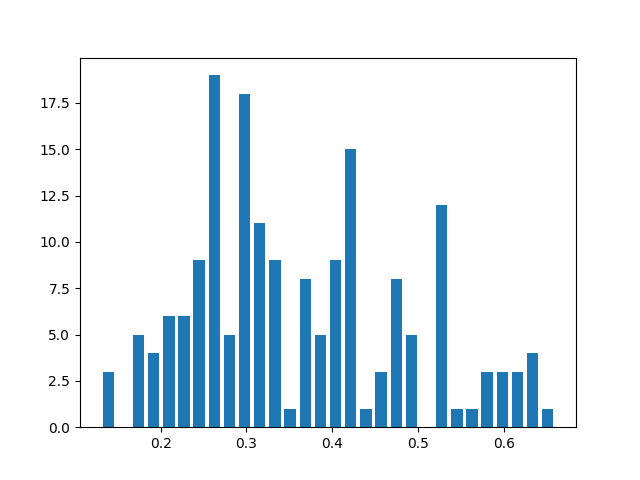
\includegraphics[width=0.2\textwidth]{img/stats/Nonflavanoid_phenols.png} \\ \hline
      Proanthocyanins &    0.41 &     3.58 &    1.59 &    0.57 &       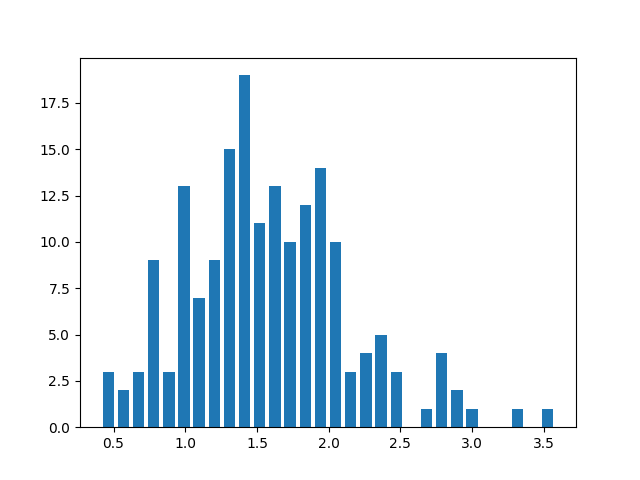
\includegraphics[width=0.2\textwidth]{img/stats/Proanthocyanins.png} \\ \hline
            Intensity &    1.28 &    13.00 &    5.06 &    2.31 &             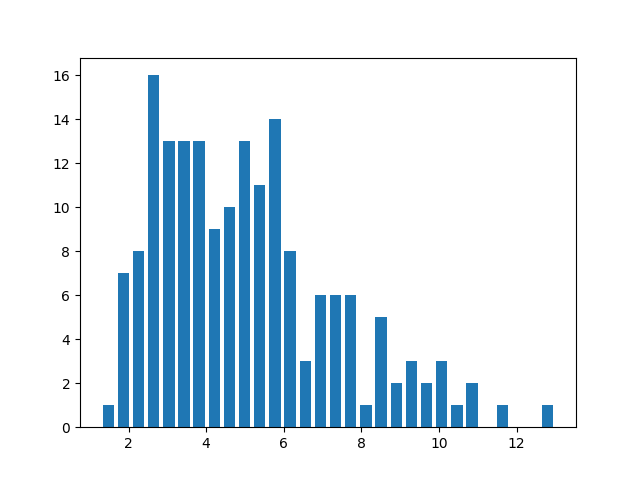
\includegraphics[width=0.2\textwidth]{img/stats/Intensity.png} \\ \hline
                  Hue &    0.48 &     1.71 &    0.96 &    0.23 &                   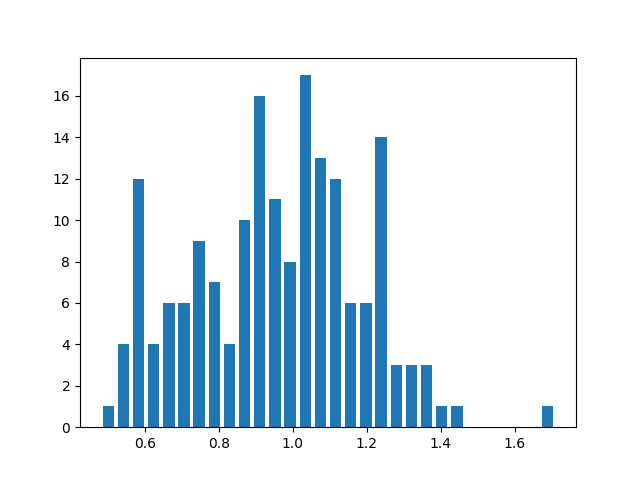
\includegraphics[width=0.2\textwidth]{img/stats/Hue.png} \\ \hline
          OD280\_OD315 &    1.27 &     4.00 &    2.61 &    0.71 &           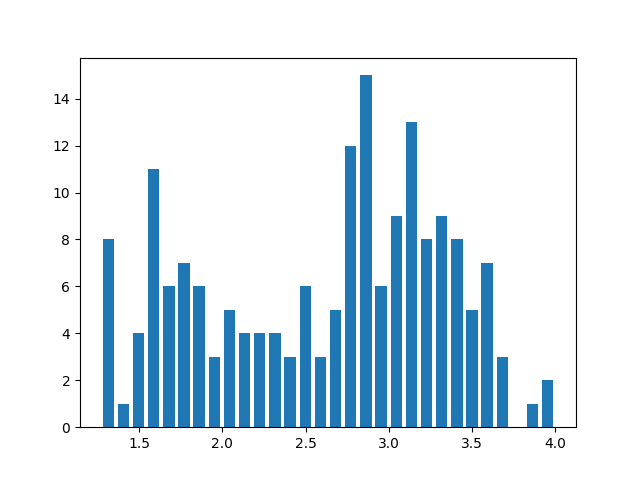
\includegraphics[width=0.2\textwidth]{img/stats/OD280_OD315.png} \\ \hline
              Proline &  278.00 &  1680.00 &  746.89 &  314.02 &               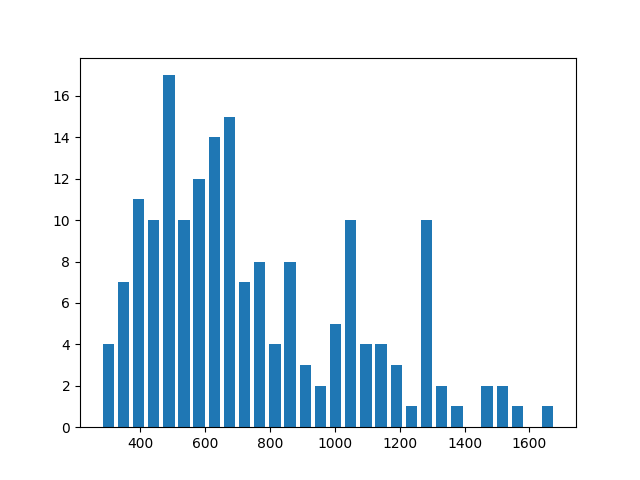
\includegraphics[width=0.2\textwidth]{img/stats/Proline.png} \\ \hline

\end{tabular} 
  \caption{Atrybuty zbioru danych "Wine".}
\end{table}
